% \vspace{-1mm}
\section{Exploring Workflow Utilization in Context and in Action}
\label{sec:expand-action}
% \vspace{-1mm}
Besides integrating workflows as agent memory, we also explore workflows in expanding the agent action space, denoted as \textsc{AWM}$_{AS}$.
We leverage the programmatic nature of workflows and wrap each workflow into a high-level function, similar to a shortcut tool the agent can call to perform a pre-determined series of actions \citep{wang2024what}.
Formally, an agent is initially equipped with default, primitive actions $P$ (\eg, \texttt{click}, \texttt{type}), and \textsc{AWM}$_{AS}$ adds the induced workflow actions $W$ (e.g., \texttt{find\_place}, \texttt{get\_place\_zipcode}) to its action space. 

The agent can call a primitive or workflow action at each step. When a primitive action is called, the agent immediately takes that action. 
When the agent calls a workflow action, it will trigger the
%
\begin{wraptable}[8]{r}{0.53\textwidth}
\small
\vspace{-4mm}
\caption{Mind2Web results with \textsc{AWM}$_{AS}$ variant that alters the action space besides memory augmentation. All methods use \texttt{gpt-4}.}
% \vspace{2mm}
\label{tab:action-space}
\begin{tabular}{l|cccc}
\toprule
{\bf Method} & {\bf Elem Acc} & {\bf Action F$_{1}$} & {\bf Step SR} & {\bf SR} \\
\midrule
{MindAct} & {41.6} & {\bf 60.6} & {36.2} & {2.0} \\
\textsc{AWM} & {50.6} & {57.3} & {45.1} & {\bf 4.8} \\
\textsc{AWM}$_{AS}$ & {\bf 51.8} & {56.7} & {\bf 46.4} & {3.6} \\
\bottomrule
\end{tabular}
\vspace{-1mm}
\end{wraptable}
%
sequence of pre-determined steps in the workflow. For example, calling the \texttt{login(username, password)} workflow action results in sequentially executing \texttt{click(box1-id)} $\rightarrow$ \texttt{type(box1-id, username)} $\rightarrow$ \texttt{click(box2-id)} $\rightarrow$ \texttt{type(box2-id, password)} $\rightarrow$ \texttt{click(submit-id)}.
The workflow action is completed when all intermediate primitive actions are finished.

In \autoref{tab:action-space}, expanding the agent action space with workflows (\textsc{AWM}$_{AS}$) slightly improves the step success rate by $1.3$ points, and gets the same overall success rate, $3.2$, of the base memory-augmented \awm. 
%
We analyzed agent predictions and found they call workflow actions in merely $18.5$\% of the tasks, suggesting a resistance of current agents to use newly-added actions. Overall, expanding actions with workflows seems to reinforce workflows in memory, and brings small extra gains as auxiliary actions.

\begin{wrapfigure}[15]{r}{0.68\textwidth}
\vspace{-7mm}
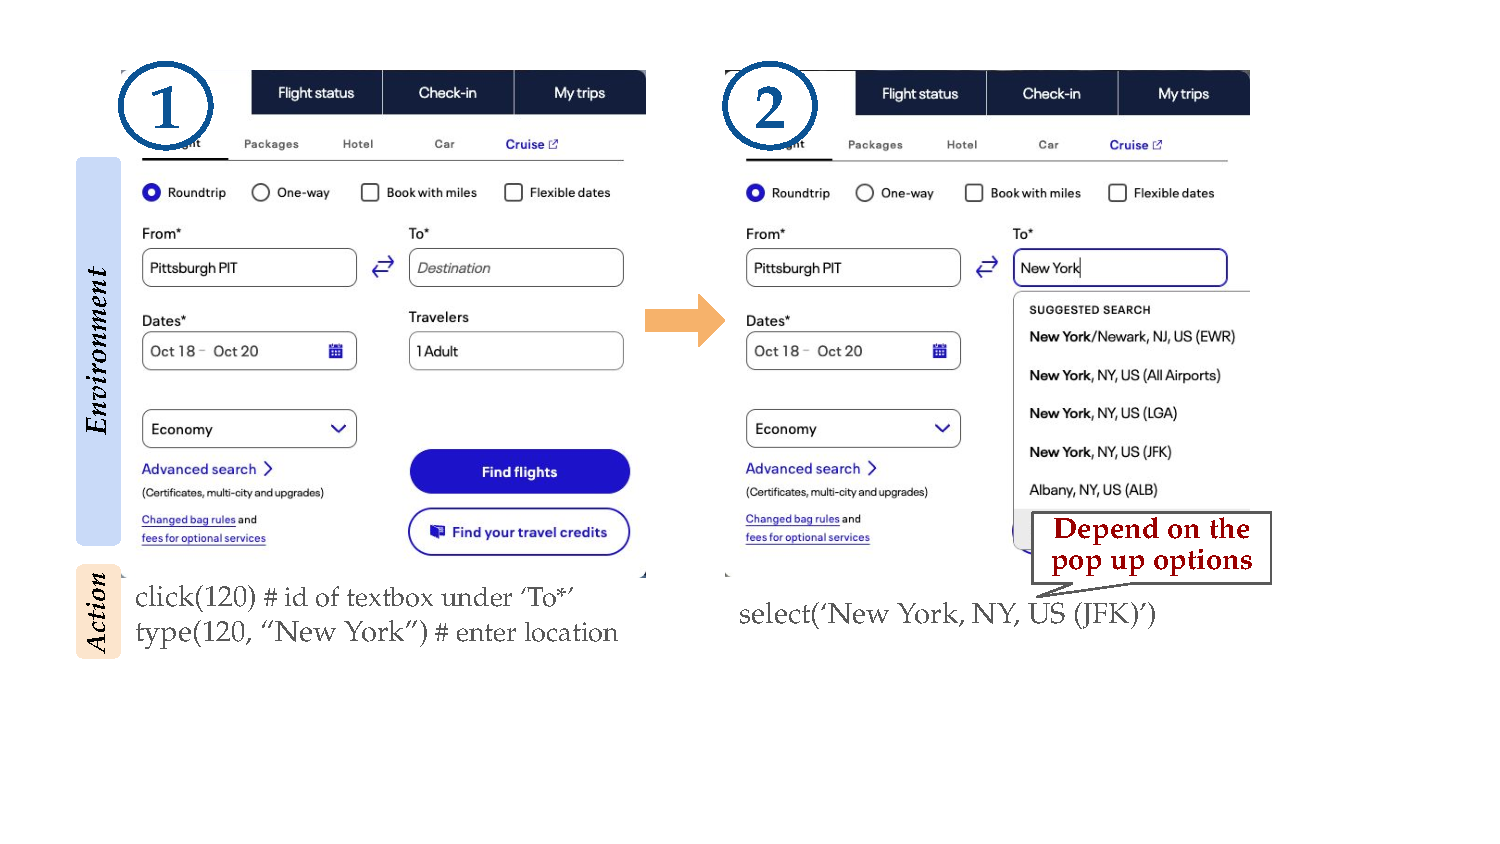
\includegraphics[width=0.67\textwidth]{./figures/action-space.pdf}
\vspace{-2mm}
\caption{An example of dynamic environment changes that challenge workflow action utilization.}
\label{fig:action-space}
% \vspace{-1mm}
\end{wrapfigure}

However, workflow actions do not always lead to task success.
A representative example is shown in \autoref{fig:action-space}. When booking flights, users often input a city name such as ``New York,'' yet the system often pops up some nearby airports to support next-step search. While one can induce a \texttt{book\_flight} workflow that enters all required data via a pre-determined action sequence, the action to choose pop-up airports is executed without seeing the intermediate states with available pop-up options, and is not flexible enough to do so. More advanced techniques such as granting real-time state access or dynamic execution loops can be promising to solve this issue, and we encourage future work to leverage the \awm framework to explore these.